\documentclass{standalone}
\usepackage{tikz}

\begin{document}

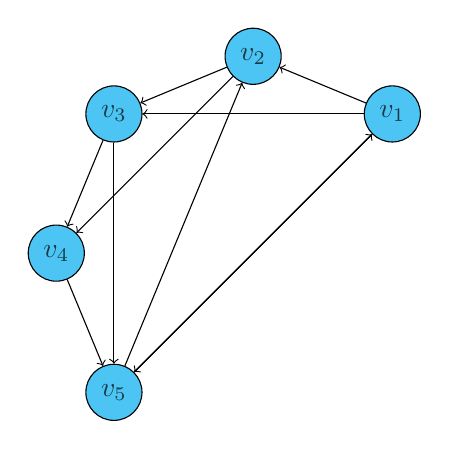
\begin{tikzpicture}
    % Define coordinates for octagon
    \coordinate (center) at (0,0);
    \foreach \i in {1,...,8} {
        \coordinate (v\i) at ({45*\i}:2.5cm);
    }
    
    % Draw nodes
    \foreach \i in {1,...,5} {
        \node[shape=circle,draw=black,fill=cyan, fill opacity=0.7] (node\i) at (v\i) {$v_{\i}$};
    }

    % Draw edges
    \foreach \i [evaluate=\i as \nextnode using {int(mod(\i,5)+1)}] in {1,...,5} {
        \draw[->] (node\i) -- (node\nextnode);
    }
    \draw[->] (node1) -- (node3);
    \draw[->] (node1) -- (node5);
    \draw[->] (node2) -- (node4);
    \draw[->] (node3) -- (node5);
    \draw[->] (node5) -- (node2);
\end{tikzpicture}

\end{document}
